\chapter{Binary neutron star mergers}\label{BNS-merg}

Neutron star mergers are one of the few laboratories in the universe where one can study phenomena such as gamma-ray emission, mass ejections, nucleosynthesis of heavy elements, gravitational waves, and the equation of state of supranuclear matter. For this reason,  observing events such as GW170817 and GW190425 has greatly interested the astrophysics and nuclear physics community in the last few years.
 
Numerical relativity simulations have shown how complicated the evolution of BNS systems is. Unlike the BBH case, matter effects play an important role in the late inspiral phase and the postmerger stage. Such simulations have also shown that the evolution of the remnant object is highly dependent on microphysics and how high its gravitational mass with respect to the maximum mass supported by the EOS of supranuclear matter. Unfortunately, nuclear physics experiments on Earth and isolated NS observations have only taken us so far, placing some constraints on it.

Given a BNS system with known masses and spins, it has been shown that using stiff and soft EOSs within current EOS bounds may produce the following scenarios for remnant:

\begin{itemize}
\item Prompt collapse to a black hole.
\item Prompt collapse to a black hole with an accretion disk.
\item Formation of a differentially rotating fluid which can be short-lived called \textit{supramassive NS} or long-lived called \textit{supramassive NS} \cite{Shibata:2019wef, Kastaun_2021}.
\end{itemize}


The following image was taken from \cite{Shibata:2019wef}. It shows how the possible outcomes listed above can be classified by comparing the total gravitational mass of the system with the EOS-dependent threshold masses for the fast collapse $M_{thr}$(see section \ref{codeon} and \cite{Kashyap_2022}) and the maximum mass for a rigidly rotating cold NS $M_{max,spin}$.



\begin{figure}[hbt!]
\begin{center}
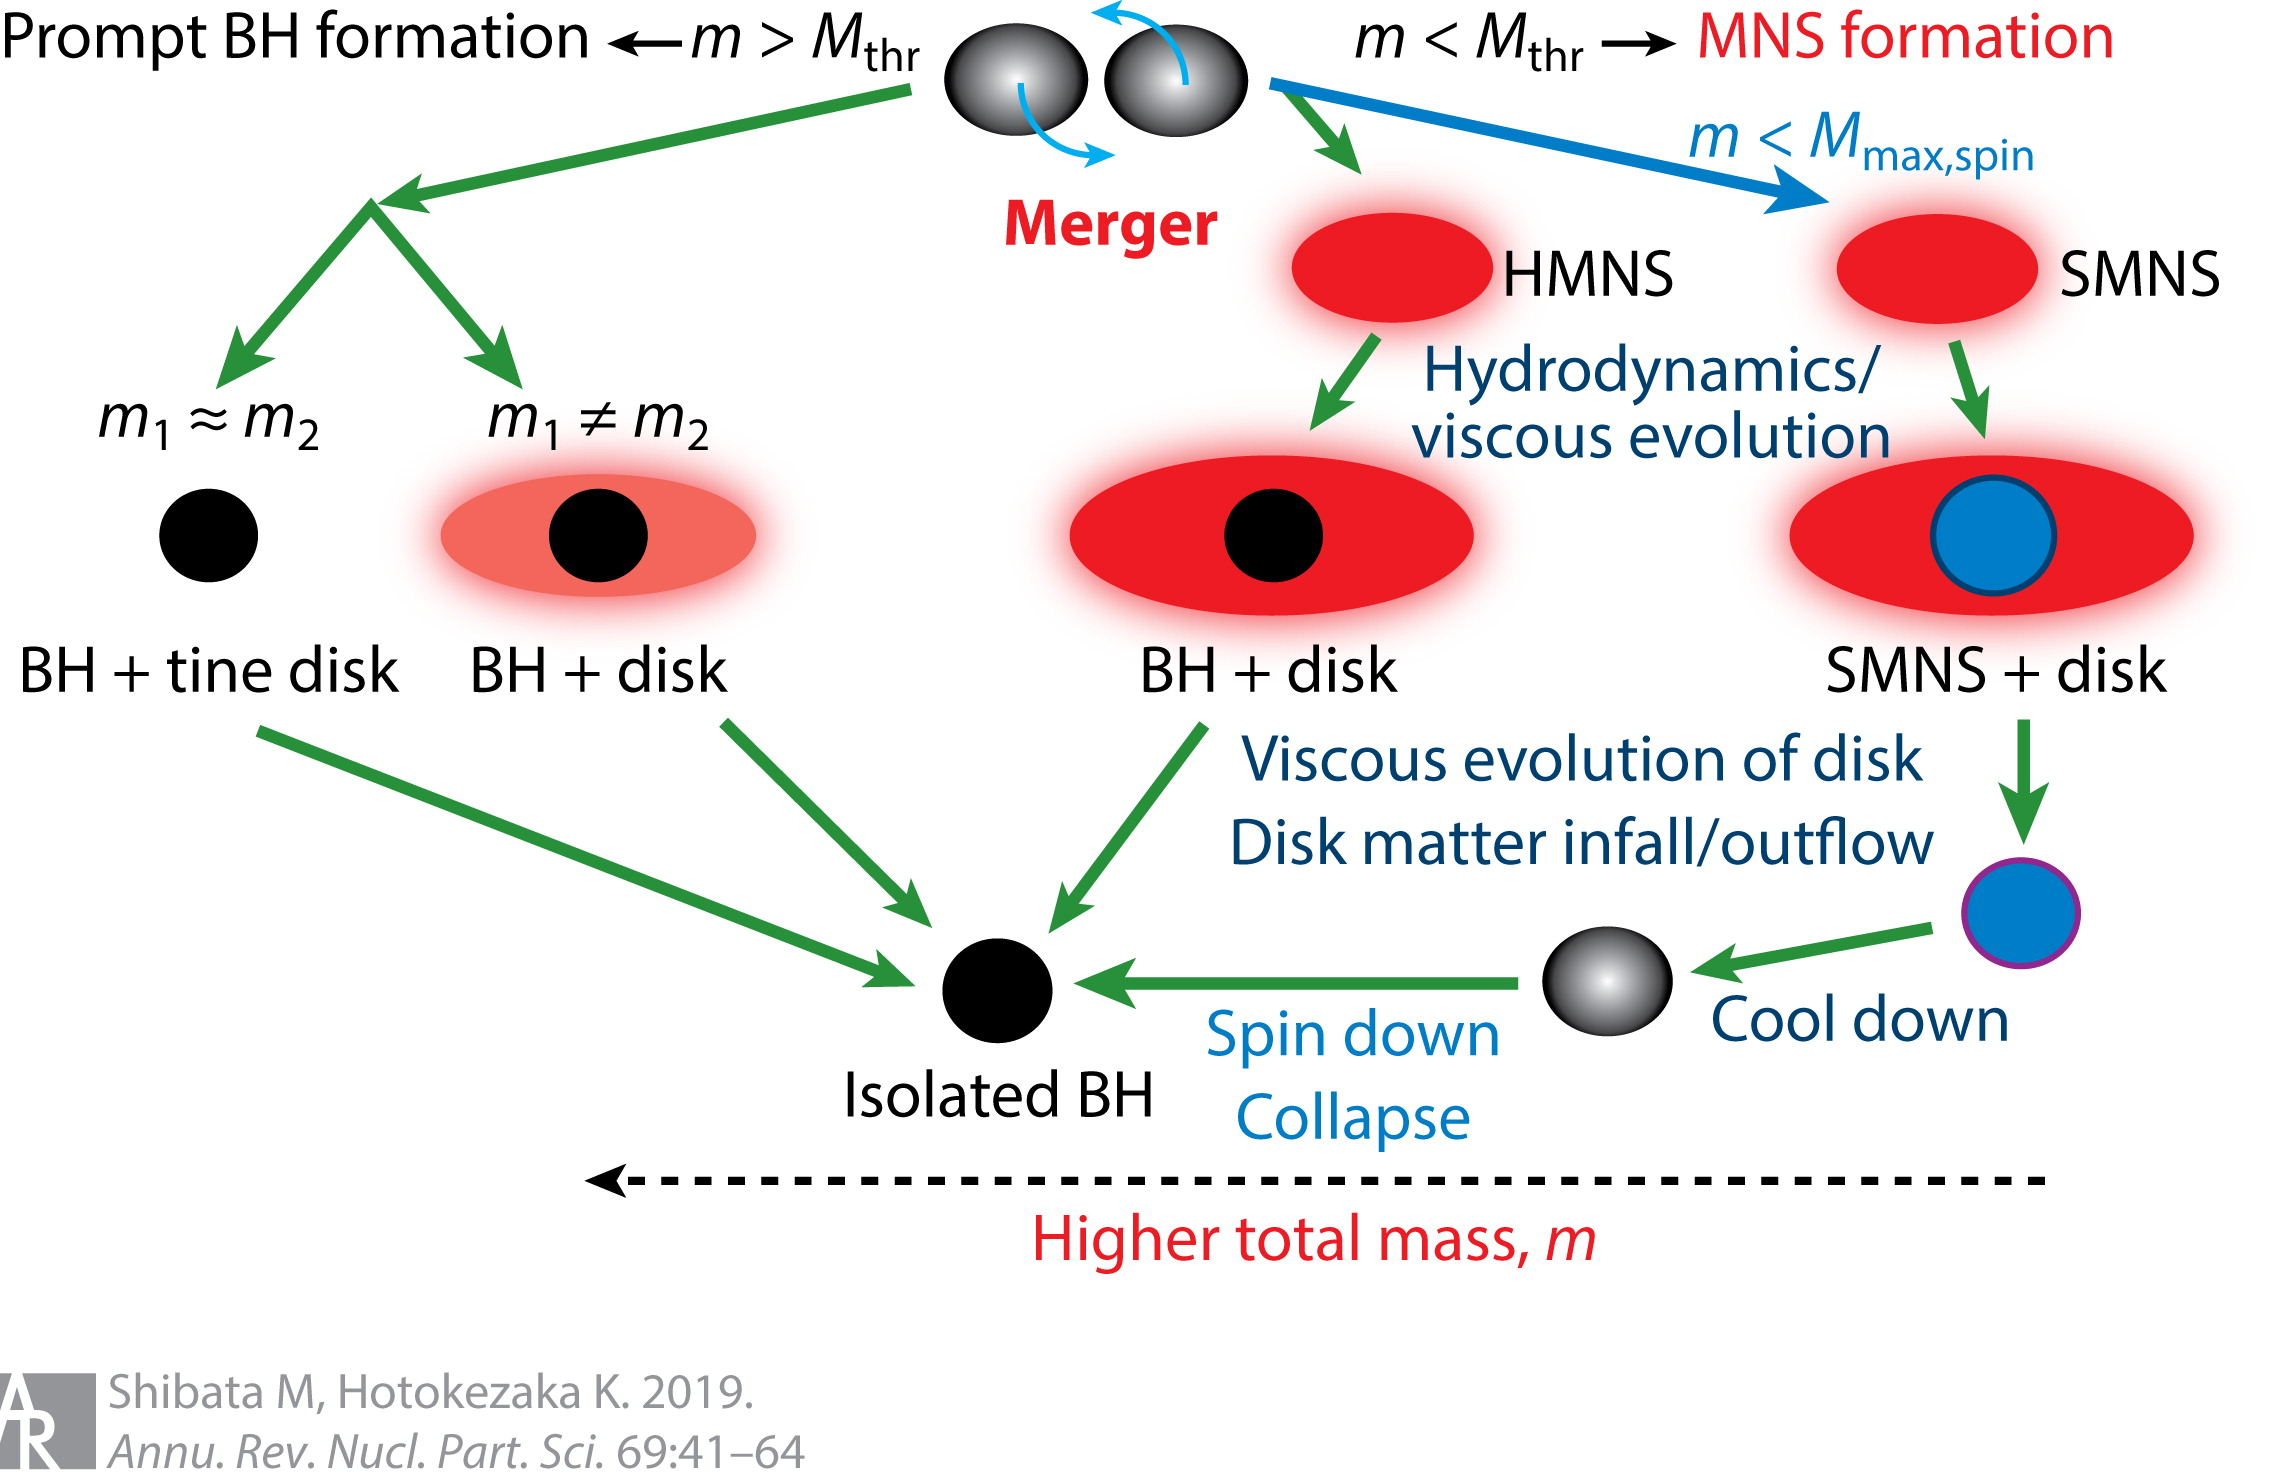
\includegraphics[width=0.5\textwidth, angle=0]{images/shi.jpeg}
\captionsetup{width=0.8\textwidth}
\caption[BNS merger remnant fate according to the EOS-dependent threshold mass]{BNS merger remnant fate according to the EOS-dependent threshold mass. This image was taken from \cite{Shibata:2019wef}. It depicts a classification of BNS postmerger remnant scenarios according to two EOS-dependent threshold masses $M_{thr}$ and $M_{max,spin}$.}
\label{BNS-out}
\end{center}
\end{figure}
\FloatBarrier

\newpage

\section{Binary neutron star waveforms}

The fact that a closed-form solution to the two-body problem closed-form in GR has not been found, implies a big difficulty when studying the GWs generated during the evolution of compact binary systems like BBH, BNS, and NSBH. For his reason, discoveries like GW150914 \cite{LIGOScientific:2016aoc}, GW170817 \cite{LIGOScientific:2017vwq}, and GW200105 \cite{LIGOScientific:2021qlt} relied on theoretical waveform models based on approximate methods like high order postnewtonian expansions, semianalytical methods like the  EOB formalism \cite{PhysRevD.96.121501,Dietrich:2018uni}, and exact waveforms extracted from numerical relativity simulations \cite{Bishop:2016lgv}.


In the present work, we will focus on BNS GW waveforms. Hence, following image is shown to depict the differences between BNS and BBH waveforms in the nonlinear regime. Notice that the BNS waveform has a more complex morphology in the postmerger phase.

\begin{figure}[hbt!]
\begin{center}
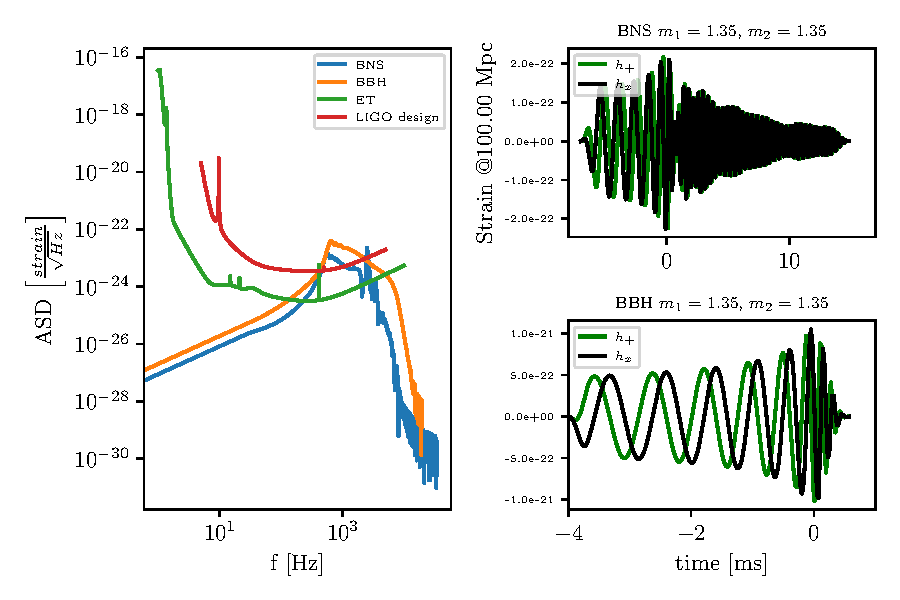
\includegraphics[width=0.6\textwidth, angle=0]{images/Data_analysis/sig_proc/BNS-BBH.pdf}
\captionsetup{width=0.8\textwidth}
\caption[Comparison of BBH and BNS GWs with the same progenitor masses]{Comparison of BBH and BNS GWs with the same progenitor masses. This figure shows GWs generated by BBH and BNS coalescenses in time domain(right) and frequency domain(left) at 100 MPc. The strain data was computed using the IMRPhenomT approximant for the BBH(lower right) \cite{Estelles:2020osj}, and the simulation BAM:0005:R01 of the CoRe BNS catalog(upper right) \cite{Dietrich:2018phi}.}
\label{BBH and BNS}
\end{center}
\end{figure}

\FloatBarrier

The complexity of the postmerger phase can be seen in the time domain after the maximum amplitude, and in the frequency domain in the kHz band, where the most dominant postmeger frequency, also called $f_2$ can be easily spotted in the amplitude spectrum. 

Although approximate analitical and semianalytical methods like the EOB formalism \cite{Damour:2012yf,PhysRevD.96.121501,Dietrich:2018uni} have got reasonably good at reproducing the GWs until the BNS late inspiral phase, the inclusion of oscillations generated by the postmerger remnant is still state-of-the-art research \cite{Breschi:2019srl, Tsang:2019esi, Soultanis:2021oia, https://doi.org/10.48550/arxiv.2205.09112}. The figure below shows how to date numerical relativity simulations are still needed to model the entire inspiral-merger-postmerger evolution.


\begin{figure}[hbt!]
\begin{center}
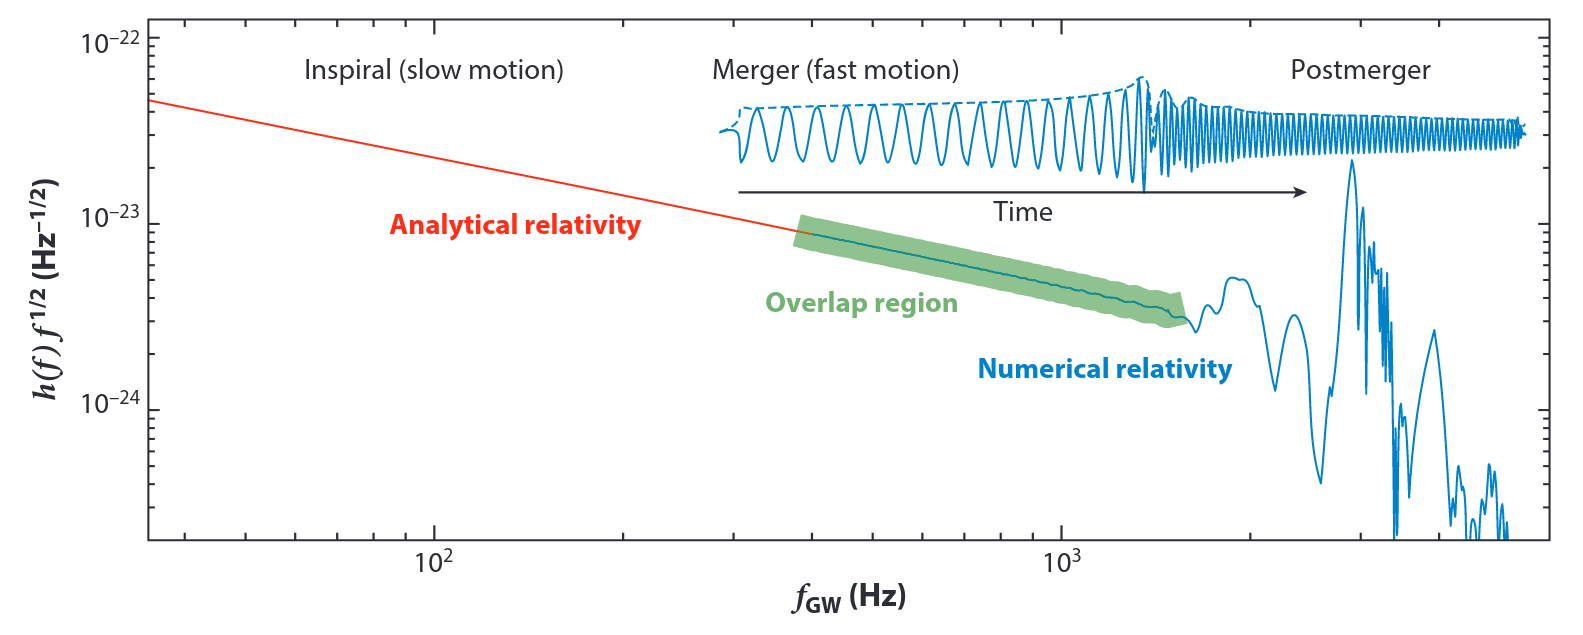
\includegraphics[width=0.6\textwidth, angle=0]{images/postmerger.png}
\captionsetup{width=0.8\textwidth}
\caption[The BNS waveform: inspiral, merger and postmerger]{The BNS waveform: inspiral, merger and postmerger. This picture was taken from \cite{Radice_2020}. It shows a BNS signal and its frequency spectrum. The waveform regions where theoretical and numerical methods are more accurate are highlighted. Notice that there is an overlapping region.}
\label{BBH and BNS2}
\end{center}
\end{figure}

\FloatBarrier

The physical parameter space of waveforms generated by a quasicircular BNS coalescence, can be entirely defined in terms of the masses of their constituents $m_1$ and $m_2$, their spins $\vec{S}_1$ and $\vec{S}_2$, and their tidal deformability $\Lambda_1$ and $\Lambda_2$\cite{Hinderer:2009ca}. However, the following derived quantities are listed below since they can be resolved much better by experiments like LIGO Virgo and KAGRA, hence they are widely used in GW astronomy.

\begin{equation}
\mathcal{M} = \frac{(m_1 m_2)^{(3/5)}}{(m_1 + m_2)^{1/5}}
\end{equation}

\begin{equation}\label{chieff}
\chi_{_{eff}} = \frac{m_1}{M}\cdot \chi_1^z + \frac{m_2}{M}\cdot \chi_2^z - \frac{38}{113} \frac{m_1 m_2}{M^2}(\chi_1^z + \chi_2^z)
\end{equation}


\begin{equation}
\tilde{\Lambda} = \frac{16}{13} \left[ \frac{(m_1 +12m_2)(m_1)^4}{M^5} \Lambda_1 + \frac{(m_2 +12m_1)(m_2)^4}{M^5} \Lambda_2 \right]
\end{equation}

Where $\chi_j = \frac{S_j}{m_j}$ is the dimensionless spin parameter, and $\Lambda_j = \frac{2k_2}{3(C_j)^5}$ accounts for the dominant effect of the tidal deformability  which depends on the $l=2$ gravitoelectric love number given by

\begin{equation}
k_l = \frac{(2l-1)!}{2}\frac{G \mu_l}{R^{2l+1}}
\end{equation}

Where coefficients $\mu_l$ result from the solution of stationary perturbations of spherical relativistic stars \cite{PhysRevD.80.084035,PhysRevD.80.084018,PhysRevD.77.021502,2020GReGr..52..108B}.

The GWs can be extracted from simulations using several methods. Some extract the Weyl scalar $\psi^4$ in coordinate spheres of finite radius $R$ \cite{Bishop:2016lgv,Thorne:1980ru} decomposing the radiation field in spin weighted spherical harmonics, and others use the Cauchy characteristic method to get the radiation field at null infinity \cite{Barkett:2019uae}.

\begin{equation}\label{pso}
R\psi^4(t) = - R(\ddot{h}_+ - i\ddot{h}_\times)(t) = \sum_{l=-2}^{\infty}  \sum_{m=-l}^{l} A_{_{_{lm}}}(t) \cdot {}_{_{_{-2}}}Y_{_{_{lm}}}(\theta, \phi)
\end{equation}

Where the coefficients $A_{lm}$ are obtained by integrating the Weyl scalar over the angular  part

\begin{equation}
A_{_{_{lm}}} = \oint \psi^4({}_{_{_{-2}}}Y^{*}_{_{_{lm}}}(\theta, \phi)) d\Omega
\end{equation}

We can integrate the Weyl scalar to obtain the metric perturbations $h$ \ref{met_pert} decomposed in spin-weighted spherical harmonics.
$ h_{lm} = - \int dt' dt'' \psi_{lm}^4$
 
\begin{equation}\label{fvr}
RH(t) = R(h_+ - ih_{\times})(t) = \sum_{l=-2}^{\infty}  \sum_{m=-l}^{l} h_{_{_{lm}}}(t) \cdot {}_{_{_{-2}}}Y_{_{_{lm}}}(\theta, \phi)
\end{equation}

\begin{mdframed}
\textbf{Remark:} keep in mind that  GW detectors observe a real-valued linear combination of $h_+$ and $h_\times$ that depends on the detector angular coordinates $\theta$ and $\phi$  and the polarization angle $\psi$ (see Sathyaprakash et al. \cite[section 4.2.1]{Sathyaprakash:2009xs})

\begin{equation}
h(t) = F^{+}(\theta, \phi, \psi) h_+(t) + F^{\times}(\theta, \phi, \psi) h_{\times}(t)
\end{equation}

\begin{equation}
\begin{aligned}
& F_{+}=\frac{1}{2}\left(1+\cos ^2 \theta\right) \cos 2 \phi \cos 2 \psi-\cos \theta \sin 2 \phi \sin 2 \psi, \\
& F_{\times}=\frac{1}{2}\left(1+\cos ^2 \theta\right) \cos 2 \phi \sin 2 \psi+\cos \theta \sin 2 \phi \cos 2 \psi
\end{aligned}
\end{equation}
\end{mdframed}


Several observables can be computed using the complex strain $H(t)$ and the complex strain components $h_{l,m}$ such as:

\begin{itemize}

\item The energy and angular momentum carried by the waves \cite{Ruiz_2007}

%\begin{equation}
%\mathcal{E}_{rad} = \lim_{r\to\infty} \frac{c^2 r^2}{16\pi G} \sum_{l=-2}^{\infty}  \sum_{m=-l}^{l} \int_{-\infty}^{t} dt'' \Biggr| \int_{-\infty}^{t''} A_{_{_{lm}}} dt' \Biggr|
%\end{equation}
%
%
%\begin{equation}
%\mathcal{J}_{z-rad} = \lim_{r\to\infty} -\frac{i \cdot c^2 r^2}{16\pi G} Im \int_{-\infty}^{t}dt'\left[ \sum_{l=-2}^{\infty} \sum_{m=-l}^{l} m  \left(\int_{-\infty}^{t'} \int_{-\infty}^{t''} dt''dt''' A_{_{_{lm}}}\right)  \cdot \left( \int_{-\infty}^{t'} dt'' (A_{_{_{lm}}})^* \right) \right]
%\end{equation}

\begin{equation}
\mathcal{E}_{rad} = \lim_{r\to\infty} \frac{c^2 r^2}{16\pi G} \sum_{l=-2}^{\infty}  \sum_{m=-l}^{l} \int_{-\infty}^{t} dt'' \Biggr|  \dot{h}_{_{_{lm}}}(t'')  \Biggr|
\end{equation}


\begin{equation}
\mathcal{J}_{z-rad} = \lim_{r\to\infty} -\frac{i \cdot c^2 r^2}{16\pi G} Im \int_{-\infty}^{t}dt'\left[ \sum_{l=-2}^{\infty} \sum_{m=-l}^{l} m  \left(h_{lm}\right)  \cdot \left( \dot{h}^*_{lm} \right) \right]
\end{equation}

\item Signal features like frequency and duration using amplitude weighted averages.

\begin{equation}\label{dwei}
d_{wei} = \frac{\int_{t_{*}}^{\infty} \left| H(t) \right| \cdot t \hspace{1mm}dt }{\int_{t_{*}}^{\infty} \left| H(t) \right| dt}
\end{equation}

\begin{equation}\label{fwei}
f_{wei} = \frac{\int_{t_{*}}^{\infty}  \left| H(t) \right| \cdot \dot{\phi}(t)  dt }{\int_{t_{*}}^{\infty} \left| H(t) \right|dt}
\end{equation}

Where $t_{*}$ its a finite time where the waveform starts, $\left| H(t) \right|$ is the strain's envelope and $\dot{\phi}(t)$ its phase velocity given by 

\begin{equation}\label{curnc}
\dot{\phi}(t)=\frac{d}{dt} \left[ \arctan \left( \frac{Im(H)}{Re(H)} \right)(t) \right]
\end{equation}

\end{itemize}



\newpage
\section{Numerical relativity waveform catalogs}\label{NR}

BNS systems have been successfully evolved on supercomputers around the world using various numerical relativity codes since the 2000s \cite{Shibata:1999hn,Shibata:1999wm,Shibata:2019wef}. Results from various authors have been collected in data sets of systems with different spins, masses, EOSs, and resolutions called NR catalogs. Unfortunately, since each simulation can take weeks on a supercomputer, mapping every point in the parameter space of a BNS to a fully relativistic simulation is a task beyond the reach of current high-performance computing facilities. For example, since the intrinsic parameters of a BNS system are the tidal deformability, spins, and masses, filling the parameter space of quasicircular BNS mergers would entail filling a discrete 6-dimensional hypercube in a sufficiently dense manner so that most regions of that space are optimally sampled. Therefore, existing catalogs are more of an unordered collection of hundreds of simulation results rather than an attempt to sample the physical parameter space of a CBC optimally. 


In particular, this thesis uses the results of two NR catalogs that sum up to about $220$ waveforms, Most of them provided by the CoRe BNS collaboration \cite{Dietrich:2018phi}, which collects the results of 160 simulations covering a wide variety of studies related to neutron star physics \cite{Bernuzzi:2014kca,Dietrich:2016hky,Bernuzzi:2016pie,Dietrich:2017aum, Dietrich:2016lyp,Dietrich:2015pxa,Dietrich:2017xqb,Radice:2017zta,Bernuzzi:2014owa,Dietrich:2015iva,Bernuzzi:2015rla, Radice:2016gym,Radice:2016rys,Radice:2017lry,Dietrich:2017feu, Zappa:2017xba}, and a collection of about 60 waveforms computed by other groups for similar purposes \cite{Maione:2016zqz, Kastaun:2016elu,Maione:2017aux,Ciolfi:2017uak,Feo:2016cbs, Kawamura:2016nmk,DePietri:2015lya,DePietri:2018tpx}.

The set of 220 simulations has been run using different numerical relativity codes such as the Einstein toolkit \cite{Loffler:2011ay,Mosta:2013gwu}, BAM \cite{PhysRevLett.92.211101,PhysRevD.77.024027,Thierfelder:2011yi}, THC \cite{Radice_2012}, and Whisky \cite{Baiotti:2003btu,Giacomazzo:2007ti} that evolve the Einstein's field equations using the 3+1 composition. In addition, LORENE \cite{lorene}, and SGRID \cite{Tichy_2009,Tichy_2012,Dietrich_2015} were used to generate the initial initial data for each BNS simulation. In the following, we will briefly describe each catalog separately.


\begin{itemize}[leftmargin=*]

\item CoRe BNS catalog (164 waveforms).

This catalog includes a dataset with a wide variety of BNS merger simulations with different resolutions, and equations of state \cite{Banik_2014,Steiner:2012rk,PhysRevD.79.124032}. It considers systems with equal masses, high mass ratios, spinning binaries, and highly eccentric systems (see appendix \ref{layer}).

The simulations use LORENE or SGRID to construct the initial data. In addition, they are run using the BSSNOK \cite{PhysRevD.52.5428,1987PThPS..90....1N,Bernuzzi_2010} or Z4c \cite{Ruiz_2011,Weyhausen_2012,Hilditch_2013} formulations to evolve spacetime and matter effects via general relativistic hydrodynamics. Simulations in this catalog use two different codes: BAM and THC. Some mergers in the catalog included the effects of EOSs with microphysics and neutrino cooling via a neutrino leakage scheme and viscous effects using the large eddy scheme GRLES \cite{Radice_2017}. It should be noted that this catalog does not include simulations with magnetic fields yet.

\item Collection of about 60 waveforms calculated by Kawamura et al. \cite{Kawamura:2016nmk}, De Petri et al. \cite{DePietri:2018tpx,DePietri:2015lya}, Feo et al. \cite{Feo:2016cbs}, Kastaun et al. \cite{Kastaun:2016elu}, Maione et al. \cite{Maione:2016zqz,Maione:2017aux} and Ciolfi et al. \cite{Ciolfi:2017uak}

This dataset covers a smaller subset of the BNS physical parameter(see appendix \ref{layer}). It contains the results of around 60 simulations with different resolutions, and equations of state \cite{PhysRevC.82.015806,PhysRevC.83.035802,PhysRevC.58.1804,PhysRevD.79.124032,PhysRevLett.67.2414,PhysRevC.52.2072}.

Most of these simulations used public codes like LORENE, the Einstein toolkit, to evolve the binary systems. Although most of these simulations do not consider magnetic fields, those computed in \cite{Kawamura:2016nmk,Ciolfi:2017uak} are an exception. 

\end{itemize}



\section{The binary neutron star postmerger waveform}

Although in recent years there has been a great interest in modeling the postmeger part of BNS GW waveforms, most models currently used in low latency searches for GW only contain the oscillations of the inspiral part \cite{Hinderer:2009ca,Damour:2012yf,PhysRevD.96.121501,Dietrich:2018uni}. The high complexity of BNS GWs in the postmeger part has made the completion of the postmeger stage of existing phenomenological approximants a complicated task. Although, at present, there are some models for the postmeger stage \cite{Breschi:2019srl, Tsang:2019esi, Soultanis:2021oia, https://doi.org/10.48550/arxiv.2205.09112}, most of them share the same problem: they require a parameter space of many dimensions. For this reason, these models are not suitable yet for use in low-latency GW search pipelines and parameter estimation runs because of their high computational cost.

For that reason, instead of using such sophisticated phenomenological approximants, the following description of the postmerger signal will be done using the sample of 220 numerical relativity waveforms described in section \ref{NR}, from the point of view of time domain signal processing.

Let us begin by describing the strain H(t) \ref{fvr} of the postmerger signal as an overmodulated complex-valued signal \cite{Kastaun:2016elu}. Such signals may have several local minima of amplitude correlated with peaks in the phase velocity \ref{curnc}. The following figure shows how such a feature can be observed the complex plane in polar coordinates, where it can be seen that as the orbits of $|H|(\phi)$ approach the origin, the orbits of $\dot{\phi}(\phi)$ reach a maximum.



\begin{figure}[hbt!]
\begin{center}
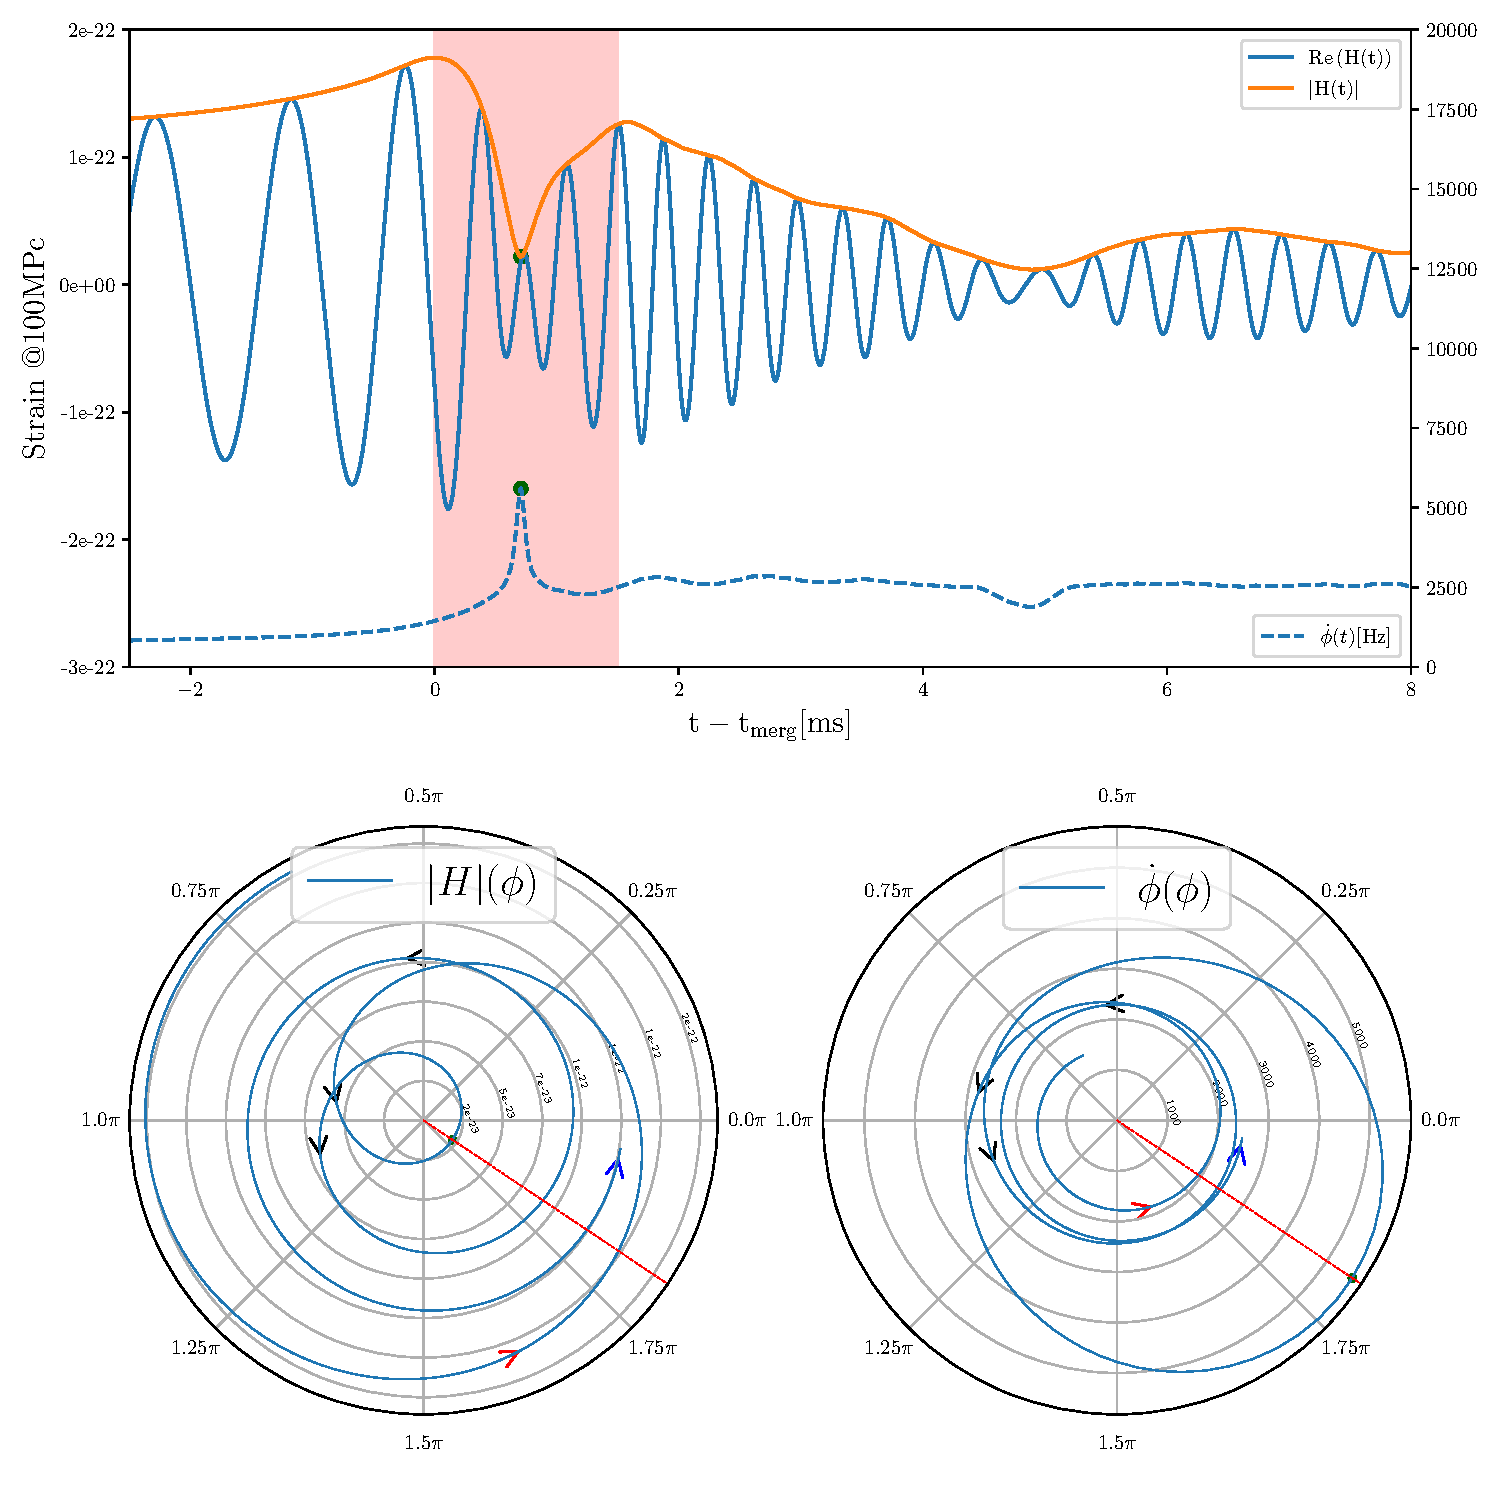
\includegraphics[width=0.8\textwidth, angle=0]{images/Data_analysis/results/postm_wf.pdf}
\end{center}
\captionsetup{width=0.8\textwidth}
\caption[The postmerger BNS signal]{The postmerger BNS signal. This figure contains the complex strain \ref{fvr} extracted from the BNS simulation BAM:0110:R01 of the CoRe catalog \cite{Dietrich:2018phi}(top). The orbits of its amplitude $|H|(\phi)$ and phase velocity $\dot{\phi}(\phi)$ are represented in the complex plane using polar coordinates (bottom). Notice that only the samples in the red shaded region(top panel) are represented in the complex plane (bottom panel) to avoid seeing too many orbits. Both polar plots contain two colored arrows to indicate time orientation. The red arrow marks earlier waveform samples, and the blue arrow marks later ones. Finally, a constant red dashed line is used to mark the phase $\phi$ at which the amplitude minima and maximum phase velocity coincide.}
\label{fig:9} 
\end{figure}

\FloatBarrier

The smooth transition between late inspiral, merger, and the postmerger phase of a BNS coalescence makes defining a starting point of a postmerger waveform a debatable subject. What is physically happening is a smooth transition from the time the atmospheres of the stars touch, and later the cores merge to produce the remnant. However, even though there is not a single time sample that marks the beginning of the postmerger phase, this work will take the maximum amplitude of the $l=2$ $m=2$ mode as such. 

The duration of the postmerger tail will be further defined by multiplying the whole BNS waveform with a rectangular window that starts at the time of  maximum amplitude of the strain's $l=2$ $m=2$ mode denoted as $t_{merg}$, and end at threshold based duration defined as follows

\begin{equation}\label{dp}
d_{postm}= \parbox{10cm}{the last time sample of the waveform with an amplitude above 5\% waveform’s maximum amplitude.}
\end{equation}


The inclusion of such a threshold is required ro avoid miscounting portions of waveform with a tail of negligible amplitude(see figure below), 

\begin{figure}[hbt!]
\begin{center}
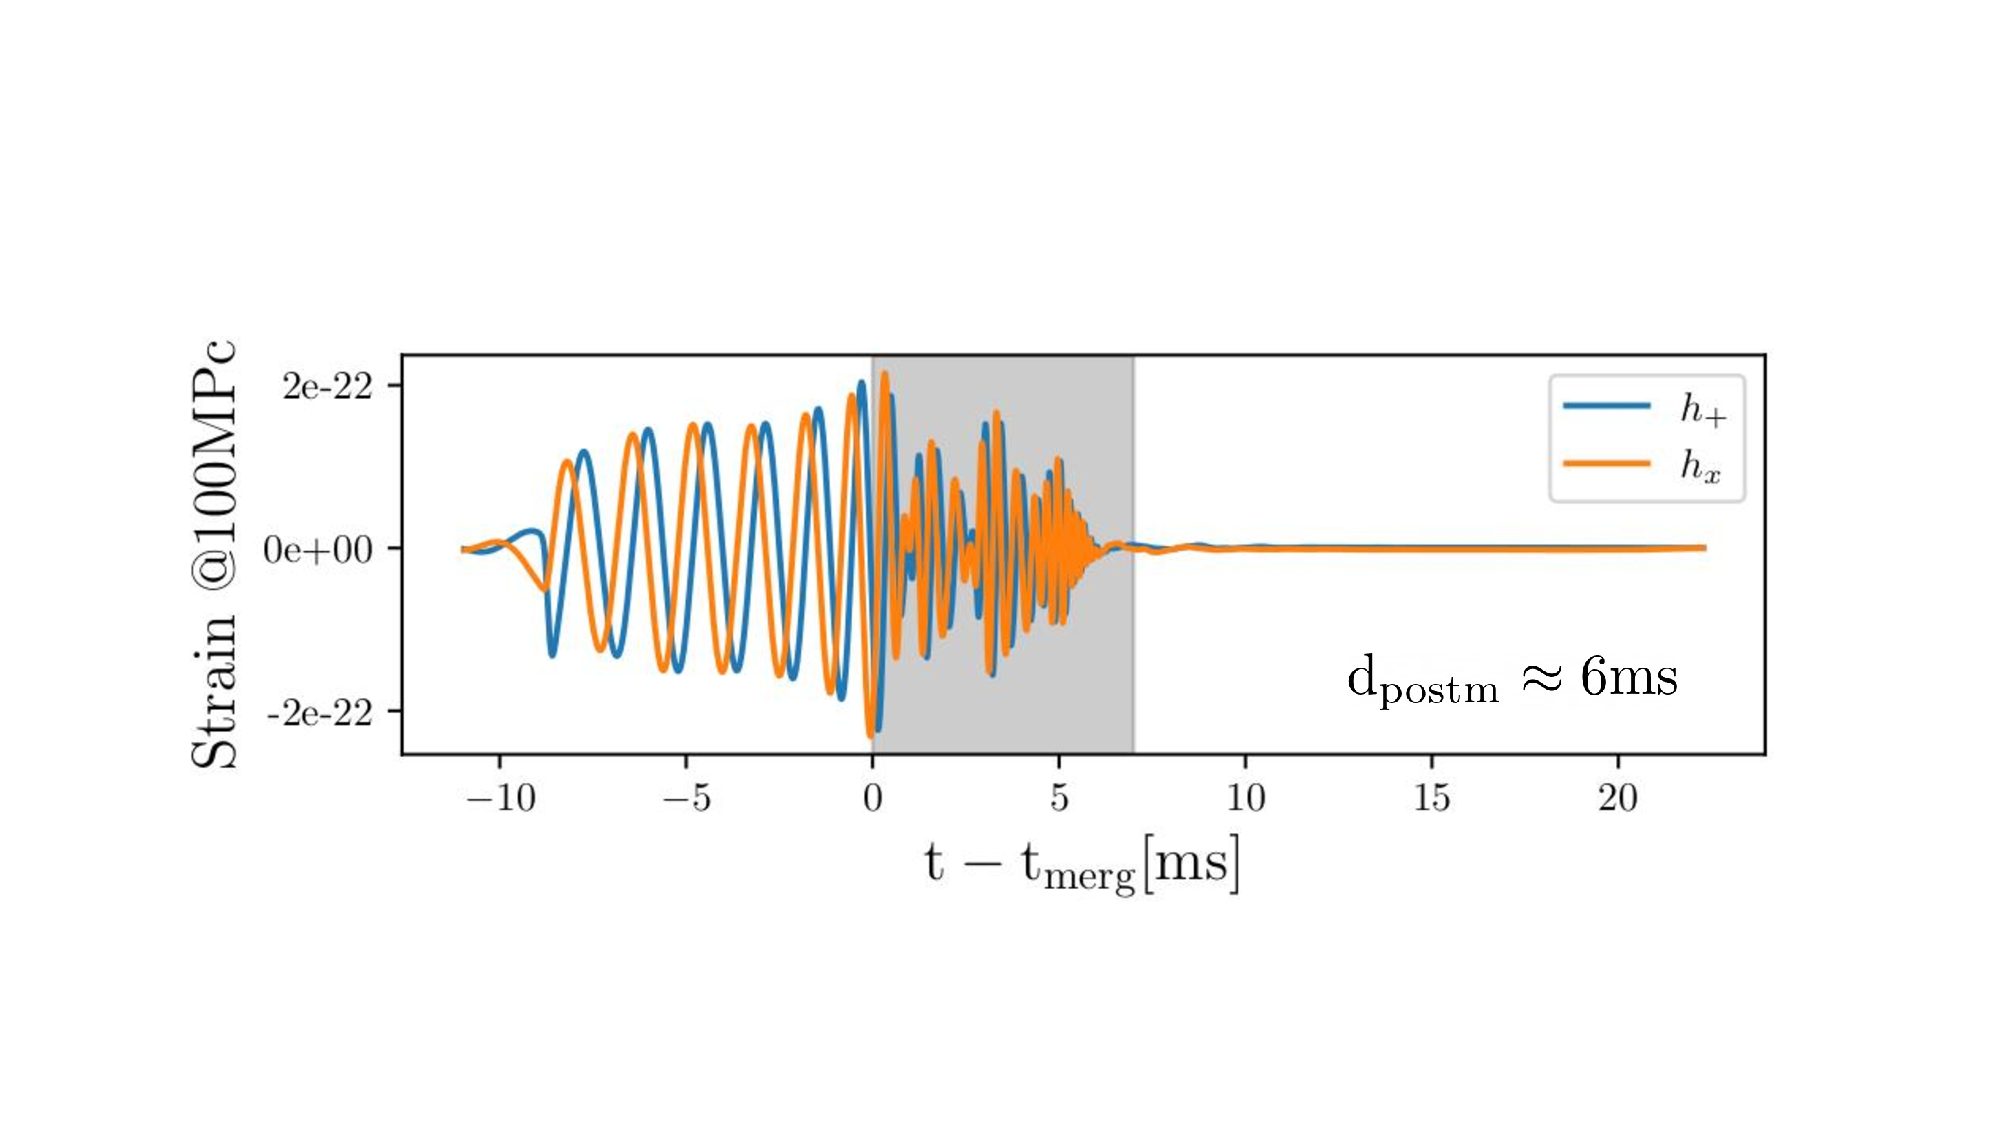
\includegraphics[width=0.9\textwidth ,trim={0 35mm 0 50mm},clip]{{images/dpostm.pdf}}
\captionsetup{width=0.8\textwidth}
\caption[The postmerger duration]{The postmerger duration. This figure depicts the region of a BNS waveform taken as the postmerger phase in this work. The strain is taken from the simulation BAM:0024:R01 of the CoRe BNS catalog \cite{Dietrich:2018phi}. Its plus and cross polarizations are represented in the time domain for a distance of 100MPc. The shaded grey area highlights the non-zero region of a rectangular window function defining the postmerger.}
\end{center}
\label{postm_cut}
\end{figure}

\FloatBarrier


Let us now take a make a rough clasification of the BNS GW postmerger waveforms present in the catalogs presented in section \ref{NR}. Even though in the waveform dataset there's a winde variety of postmerger morphologies depending on the input physics one considers., we try making the following  classification according to their duration, number of amplitude minima, and some other features that are easy to identify.



\begin{itemize}
\item Equal mass systems ($q=1$) with low total gravitational mass ($\delta=\frac{M}{M_{TOV}}<1.6$). Such systems show only one deep amplitude minimum after the merger, followed by a tail of similar amplitude.

\item Systems with high mass ratio ($q>1.5$). Such systems show at least one loud signal cycle after the merger, followed by a long low amplitude tail.

\item Spinning systems ($\chi_{eff}>0.2$). Such systems show several amplitude minima and a tail with similar amplitude.

\item Systems with high total gravitational mass ($\delta=\frac{M}{M_{TOV}}>1.6$). Such systems have a short high frequency signal.

\item Highly eccentric systems ($e>0.4$). These systems may show several cycles before the first minimum, followed by a tail with a similar amplitude.

\item Equal mass systems where viscous hydrodynamics is taken into account show a postmerger tail with stronger amplitude modulation.

\end{itemize}


\begin{figure}[hbt!]
\begin{center}
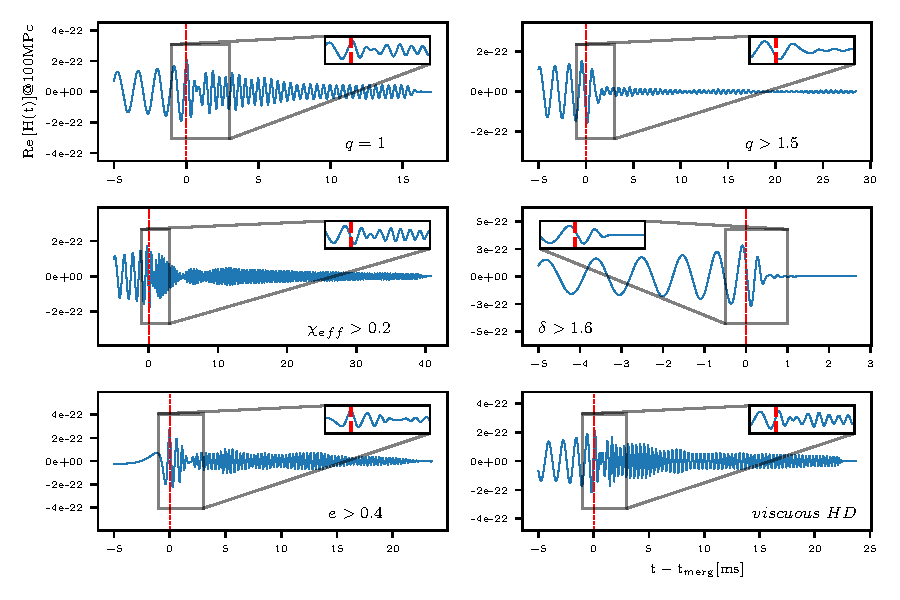
\includegraphics[width=0.8\textwidth, angle=0]{images/Data_analysis/results/postm_wf_grid.pdf}
\captionsetup{width=0.8\textwidth}
\caption[Possible BNS postmerger GW morphologies]{Possible BNS postmerger GW morphologies. This figure shows the strain in the time domain for six different example waveform morphologies in the CoRe BNS catalog\ref{Dietrich:2018phi}. If the figure is read as a matrix, plot 11 shows an equal mass system (BAM:0035, $q=m_1/m_2=1$), plot 12 a system with a high mass ratio (BAM:0094, $q=m_1/m_2>1.6$), plot 21 a highly spinning system (BAM:0110, $\chi_{_{eff}}>0.2$), plot 22 a heavy system (BAM:0001, $\delta=\frac{(m_1+m_2)}{M_{TOV}}>1.6$), the plot 31 a highly eccentric system (BAM:0115, $e>0.4$) and the plot 32 a BNS simulation for an equal mass system that included viscous hydrodynamics (THC:0019).}
\end{center}
\label{fig:10}
\end{figure}

\FloatBarrier 


Moreover, by reading physical observables from simulation metadata such as masses and mass ratios (see appendix \ref{layer}), we can examine for example whether this waveform dataset shows a correlation between these physical parameters and the duration of the postmerger phase, as implied by some of the gravitationally collapsing remnant scenarions shown in figure \ref{BNS-out}. 

\begin{figure}[hbt!]
\begin{center}
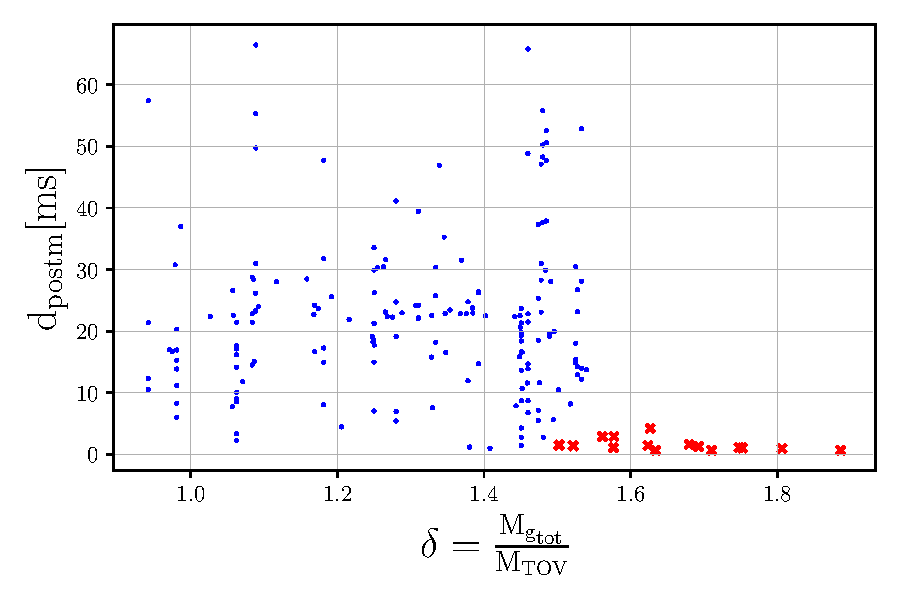
\includegraphics[width=0.65\textwidth, angle=0]{images/Data_analysis/results/res0.pdf}
\captionsetup{width=0.8\textwidth}
\caption[Can heavy systems have a long postmerger duration?]{Can heavy systems have a long postmerger duration? This scatterplot shows that for the 220 waveform dataset described in section \ref{NR}, we observe the existence of a BNS threshold mass above which the postmerger duration \ref{dp} is always below five milliseconds \cite{Kashyap_2022}. The threshold mass in this plot is measured in terms of the ratio of the BNS total gravitational mass and the maximum TOV mass \ref{delta} for a given EOS.}
\label{heavy systems}
\end{center}
\end{figure}
\FloatBarrier

Where we can clearly see the existence of a threshold mass at $\delta> 1.6$, for BNS systems generate waveforms shorter than five milliseconds.

In addition, the few waveforms with mass ratio greater than 1.6 have a very small amplitude weighted duration \ref{dwei}. Which is consistent with waveforms with a long low-amplitude tail, as the high mass ratio example shown in figure \ref{}.


\begin{figure}[hbt!]
\begin{center}
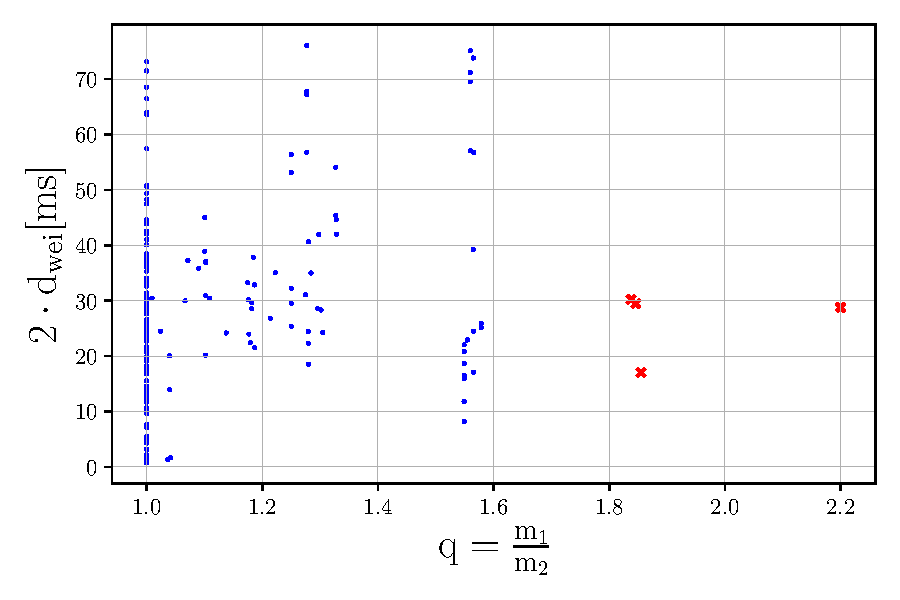
\includegraphics[width=0.65\textwidth, angle=0]{images/Data_analysis/results/Mr.pdf}
\captionsetup{width=0.8\textwidth}
\caption[The amplitude weighted duration of a high mass ratio waveform]{The amplitude weighted duration of a high mass ratio waveform. This picture shows the correlation between the high mass ratio (q>1.6) and small $d_{wei}$ \ref{dwei} observed in the waveform dataset presented in section \ref{NR} (see Kolsch et al. \cite{Kolsch:2021lub}). The red crosses highlight that all waveforms with $q>1.6$ have a weighted duration below fifteen milliseconds.}
\label{High mass ratio}
\end{center}
\end{figure}
\FloatBarrier


Moreover, we can compare the amplitude weighted averages $d_{wei}$ \ref{dwei} and $f_{wei}$ \ref{fwei}, with the postmerger's duration $d_{postm}$ and most dominant frequency $f_2$, to determine whether there's a clear correlation between them.

The following two plots show, a clear correlation among those quantities, except for certain outlier waveforms that deviate from the main clustering pattern. 

\begin{figure}[hbt!]
\begin{center}
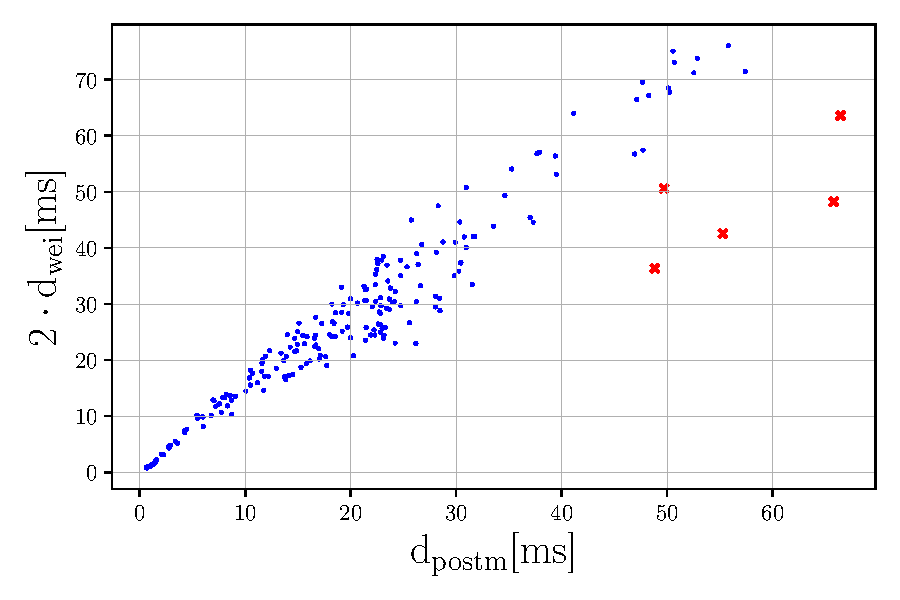
\includegraphics[width=0.6\textwidth, angle=0]{images/Data_analysis/results/res1.pdf}
\captionsetup{width=0.8\textwidth}
\caption[The postmerger amplitude weighted duration]{The postmerger amplitude weighted duration. This scatterplot examines whether the threshold-based duration \ref{dp} coincides with the values of amplitude-weighted duration \ref{dwei} for the waveform dataset presented in section \ref{NR}. The waveforms generated by highly eccentric BNS systems are highlighted using red crosses.}
\label{duration measure}
\end{center}
\end{figure}

\newpage
In the case of $d_{wei}$, the signals that deviate the most from the main straight line are highly eccentric simulations. On the other hand, looking at  $f_{wei}$ the outliers are high mass ratio simulations.

\begin{figure}[hbt!]
\begin{center}
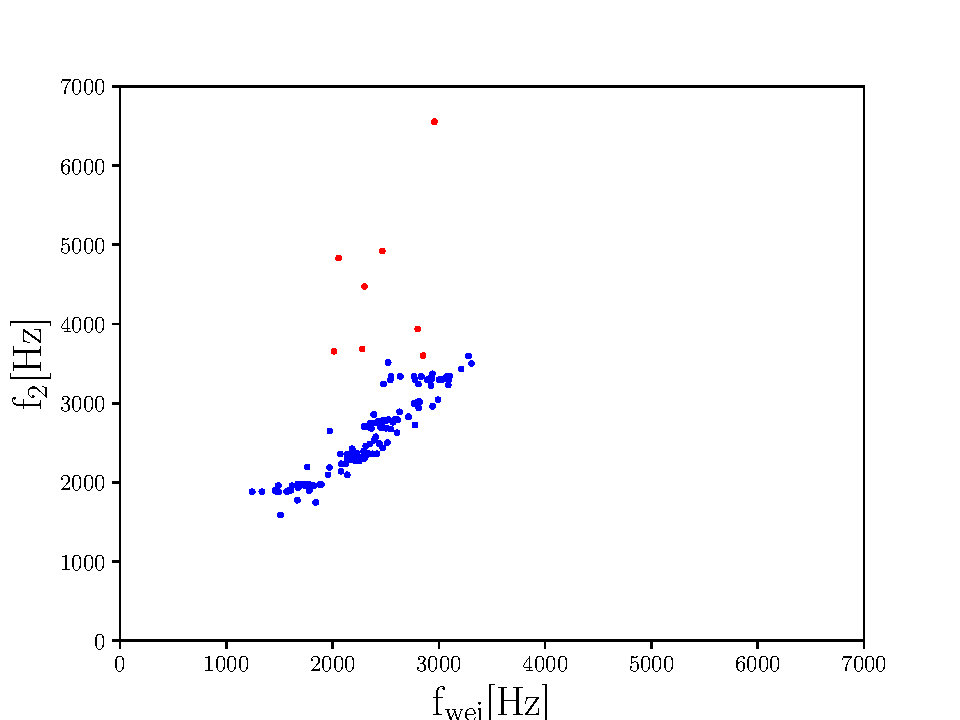
\includegraphics[width=0.6\textwidth, angle=0]{images/Data_analysis/results/f2.pdf}
\captionsetup{width=0.8\textwidth}
\caption[The postmerger amplitude weighted frequency]{The postmerger amplitude weighted frequency. This scatterplot examines whether the main postmerger frequency $f_2$ coincides with the amplitude weighted frequency \ref{fwei} for all waveforms in the CoRe BNS catalog (see section \ref{NR}). BNS systems with high mass ratio are highlighted by using red dots.}
\label{duration measure}
\end{center}
\end{figure}

\FloatBarrier








